% This is "sig-alternate.tex" V2.1 April 2013
% This file should be compiled with V2.8 of "sig-alternate.cls" May 2012
%
% This example file demonstrates the use of the 'sig-alternate.cls'
% V2.8 LaTeX2e document class file. It is for those submitting
% articles to ACM Conference Proceedings WHO DO NOT WISH TO
% STRICTLY ADHERE TO THE SIGS (PUBS-BOARD-ENDORSED) STYLE.
% The 'sig-alternate.cls' file will produce a similar-looking,
% albeit, 'tighter' paper resulting in, invariably, fewer pages.
%
% ----------------------------------------------------------------------------------------------------------------
% This .tex file (and associated .cls V2.8) produces:
%       1) The Permission Statement
%       2) The Conference (location) Info information
%       3) The Copyright Line with ACM data
%       4) NO page numbers
%
% as against the acm_proc_article-sp.cls file which
% DOES NOT produce 1) thru' 3) above.
%
% Using 'sig-alternate.cls' you have control, however, from within
% the source .tex file, over both the CopyrightYear
% (defaulted to 200X) and the ACM Copyright Data
% (defaulted to X-XXXXX-XX-X/XX/XX).
% e.g.
% \CopyrightYear{2007} will cause 2007 to appear in the copyright line.
% \crdata{0-12345-67-8/90/12} will cause 0-12345-67-8/90/12 to appear in the copyright line.
%
% ---------------------------------------------------------------------------------------------------------------
% This .tex source is an example which *does* use
% the .bib file (from which the .bbl file % is produced).
% REMEMBER HOWEVER: After having produced the .bbl file,
% and prior to final submission, you *NEED* to 'insert'
% your .bbl file into your source .tex file so as to provide
% ONE 'self-contained' source file.
%
% ================= IF YOU HAVE QUESTIONS =======================
% Questions regarding the SIGS styles, SIGS policies and
% procedures, Conferences etc. should be sent to
% Adrienne Griscti (griscti@acm.org)
%
% Technical questions _only_ to
% Gerald Murray (murray@hq.acm.org)
% ===============================================================
%
% For tracking purposes - this is V2.0 - May 2012

\documentclass{sig-alternate}

\setlength{\paperheight}{11in}
\setlength{\paperwidth}{8.5in}
\usepackage[
  pass,% keep layout unchanged 
  % showframe,% show the layout
]{geometry}

\begin{document}

% Copyright
\setcopyright{waclicense}


%% DOI
%\doi{10.475/123_4}
%
%% ISBN
%\isbn{123-4567-24-567/08/06}
%
%%Conference
%\conferenceinfo{PLDI '13}{June 16--19, 2013, Seattle, WA, USA}
%
%\acmPrice{\$15.00}

%
% --- Author Metadata here ---
\conferenceinfo{Web Audio Conference WAC-2017,}{August 21--23, 2017, London, UK.}
\CopyrightYear{2017} % Allows default copyright year (20XX) to be over-ridden - IF NEED BE.
%\crdata{0-12345-67-8/90/01}  % Allows default copyright data (0-89791-88-6/97/05) to be over-ridden - IF NEED BE.
% --- End of Author Metadata ---

\title{A collaborative web platform for sound archives management and analysis}
%\subtitle{[Extended Abstract]
%\titlenote{A full version of this paper is available as
%\textit{Author's Guide to Preparing ACM SIG Proceedings Using
%\LaTeX$2_\epsilon$\ and BibTeX} at
%\texttt{www.acm.org/eaddress.htm}}}
%
% You need the command \numberofauthors to handle the 'placement
% and alignment' of the authors beneath the title.
%
% For aesthetic reasons, we recommend 'three authors at a time'
% i.e. three 'name/affiliation blocks' be placed beneath the title.
%
% NOTE: You are NOT restricted in how many 'rows' of
% "name/affiliations" may appear. We just ask that you restrict
% the number of 'columns' to three.
%
% Because of the available 'opening page real-estate'
% we ask you to refrain from putting more than six authors
% (two rows with three columns) beneath the article title.
% More than six makes the first-page appear very cluttered indeed.
%
% Use the \alignauthor commands to handle the names
% and affiliations for an 'aesthetic maximum' of six authors.
% Add names, affiliations, addresses for
% the seventh etc. author(s) as the argument for the
% \additionalauthors command.
% These 'additional authors' will be output/set for you
% without further effort on your part as the last section in
% the body of your article BEFORE References or any Appendices.

\numberofauthors{2} %  in this sample file, there are a *total*
% of EIGHT authors. SIX appear on the 'first-page' (for formatting
% reasons) and the remaining two appear in the \additionalauthors section.
%
\author{
% You can go ahead and credit any number of authors here,
% e.g. one 'row of three' or two rows (consisting of one row of three
% and a second row of one, two or three).
%
% The command \alignauthor (no curly braces needed) should
% precede each author name, affiliation/snail-mail address and
% e-mail address. Additionally, tag each line of
% affiliation/address with \affaddr, and tag the
% e-mail address with \email.
%
% 1st. author
\alignauthor
Thomas Fillon\\
       \affaddr{Parisson}\\
       \affaddr{Paris, France}\\
       \email{thomas@parisson.com}
% 2nd. author
\alignauthor
Guillaume Pellerin\\
       \affaddr{Parisson / IRCAM}\\
       \affaddr{Paris, France}\\
       \email{guillaume.pellerin@parisson.com}
}
% There's nothing stopping you putting the seventh, eighth, etc.
% author on the opening page (as the 'third row') but we ask,
% for aesthetic reasons that you place these 'additional authors'
% in the \additional authors block, viz.

% Just remember to make sure that the TOTAL number of authors
% is the number that will appear on the first page PLUS the
% number that will appear in the \additionalauthors section.

\maketitle
\begin{sloppypar}
\begin{abstract}
In the context of digital sound archives, an innovative web framework for automatic analysis and manual annotation of audio files has been developed. This web framework, is called Timeside and is available under an open-source license.

The TimeSide framework associates an audio processing engine, an audio database, a web API and a client-side multimedia player.

The audio processing engine is written in Python language and has been designed for speech and audio signal analysis and Music Information Retrieval (MIR) tasks. It includes a set of audio analysis plugins and additionally wraps several state-of-the-art audio features extraction libraries to provide automatic annotation, segmentation and Music Information Retrieval analysis. It also provides decoding and encoding methods for most common multimedia formats.

The audio database application is handled through Django (Python) and is interfaced with the audio processing engine.

The web API component provides these functionalities over the web to enable web client to run analysis on the sounds in the audio database.
Last but not least, the multimedia player provides an web player associated with several sound and analysis visualizations together with an annotations editor through a multi-tracks display.


The TimeSide platform is available as an open-source project at the following addresses:

TimeSide: \url{https://github.com/Parisson/TimeSide}

\end{abstract}


%
% The code below should be generated by the tool at
% http://dl.acm.org/ccs.cfm
% Please copy and paste the code instead of the example below. 
%
%\begin{CCSXML}
%<ccs2012>
 %<concept>
  %<concept_id>10010520.10010553.10010562</concept_id>
  %<concept_desc>Computer systems organization~Embedded systems</concept_desc>
  %<concept_significance>500</concept_significance>
 %</concept>
 %<concept>
  %<concept_id>10010520.10010575.10010755</concept_id>
  %<concept_desc>Computer systems organization~Redundancy</concept_desc>
  %<concept_significance>300</concept_significance>
 %</concept>
 %<concept>
  %<concept_id>10010520.10010553.10010554</concept_id>
  %<concept_desc>Computer systems organization~Robotics</concept_desc>
  %<concept_significance>100</concept_significance>
 %</concept>
 %<concept>
  %<concept_id>10003033.10003083.10003095</concept_id>
  %<concept_desc>Networks~Network reliability</concept_desc>
  %<concept_significance>100</concept_significance>
 %</concept>
%</ccs2012>  
%\end{CCSXML}
%
%\ccsdesc[500]{Computer systems organization~Embedded systems}
%\ccsdesc[300]{Computer systems organization~Redundancy}
%\ccsdesc{Computer systems organization~Robotics}
%\ccsdesc[100]{Networks~Network reliability}
%
%
%%
%% End generated code
%%
%
%%
%%  Use this command to print the description
%%
%\printccsdesc
%
%% We no longer use \terms command
%%\terms{Theory}
%
%\keywords{ACM proceedings, \LaTeX, text tagging}

\section{Introduction}
In the context of digital sound archives management, researchers and archivists have expressed the need for computational tools to help them manage and analyze their archives.

For this purpose, an innovative web framework for automatic analysis and manual annotation of audio files has been developed. This web framework, is called Timeside and is developed under an open-source license in a joint collaboration between MIR \& Humanities researchers, software developers and archivists.

The TimeSide framework associates four main componnts :
an audio processing engine, 
an audio database management system, 
a web API 
and a client-side multimedia player.


\section{Audio processing engine}
The audio processing engine is written in Python language and has been designed for speech and audio signal analysis and Music Information Retrieval (MIR) tasks. It includes a set of audio analysis plugins and additionally wraps several state-of-the-art audio features extraction libraries to provide automatic annotation, segmentation and Music Information Retrieval analysis. It also provides decoding and encoding methods for most common multimedia formats.
It includes most commonly used python packages for data science and provides convenient Jupyter (ipython) notebook interface for developers and computer science researchers.

The TimeSide engine architecture is composed of several modules and makes it easy to develop and add new plugins.
\section{Audio database}
The audio database application is handled through Django (Python) and is interfaced with the audio processing engine. 
It enable to deal with the basic metadata associated with multimedia files and also is used to store the information about audio analysis (state, parameters, versioning).
Several analysis can be grouped and organized in experiments and be run over a selection of items (corpus). The management of the audio corpus together with associated metadata available through the same database or linked through another database containing further metadata (e.g. cultural or musical metadata) enables to extract or manage semantic information both from automatic content analysis and from contextual metadata.
The database models also provide tools for time-segment annotation of the multimedia items. 
Both database objects and analysis methods can be managed together through Timeside. 

\section{Web API and multimedia player}
The audio engine and the database functionalities are fully accessible through a Web API.
This API is associated with an embeddable web multimedia player. 
This multimedia player is fully compatible with HTML5 and use web audio API components. 
 It can display several sound visualizations such as waveform or time-frequency representations. It can also simultaneously displays results of automatic analysis and further enable to tune the analysis parameters. Analysis are displayed in a multitracks fashion together with manual annotations. Indeed, the web player also acts as an annotation editor and gives the possibility for user to collaboratively annotate and share time-segments piece of multimedia files.
 \begin{figure}[h]
   \centering
   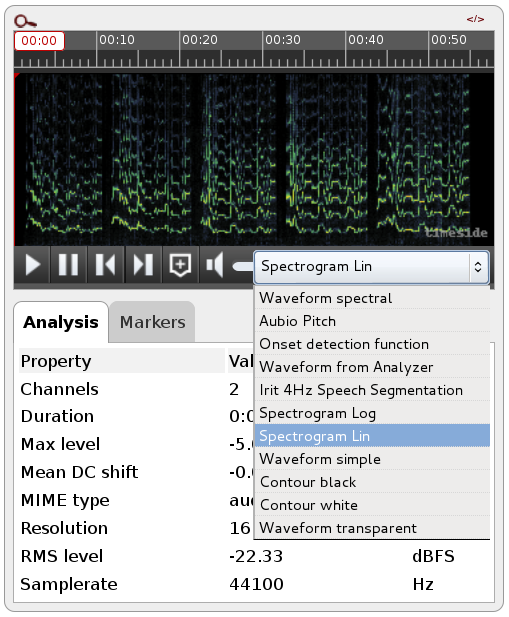
\includegraphics[width=5cm]{../../Common/img/sound_representation.png}
   
   \caption{Timeside player with various sound representations.}
\label{fig:sound_repr}
\end{figure}
\section{Applications in the case of Ethnomusicological sound archives}
The Timeside framework is a part of a larger Digital assets management framework for sound archives, the Telemeta framework, also available under an open-source license. Telemeta is a web audio platform for the management and the access to digital sound archives and audio metadata. It is developed since 2007 in the context of a collaboration between Parisson, a company, and the Center of Research in EthnoMusicology (CREM) in France.

Telemeta focuses on the enhanced and collaborative user-experience in accessing audio items and their associated metadata and on the possibility for the expert users to further enrich those metadata though hierarchical and structured fields, thesaurus and ontologies.
This platform has been deployed since 2011 in the context of ethnomusicological archives and hold the archives of the CREM\footnote{\url{http://archives.crem-cnrs.fr}}. The platform is fully operational and is now used on a daily basis by researchers, teachers and archivists in the fields of ethnomusicology, anthropology, linguistics and acoustics.

\begin{figure}[h]
  \centering
  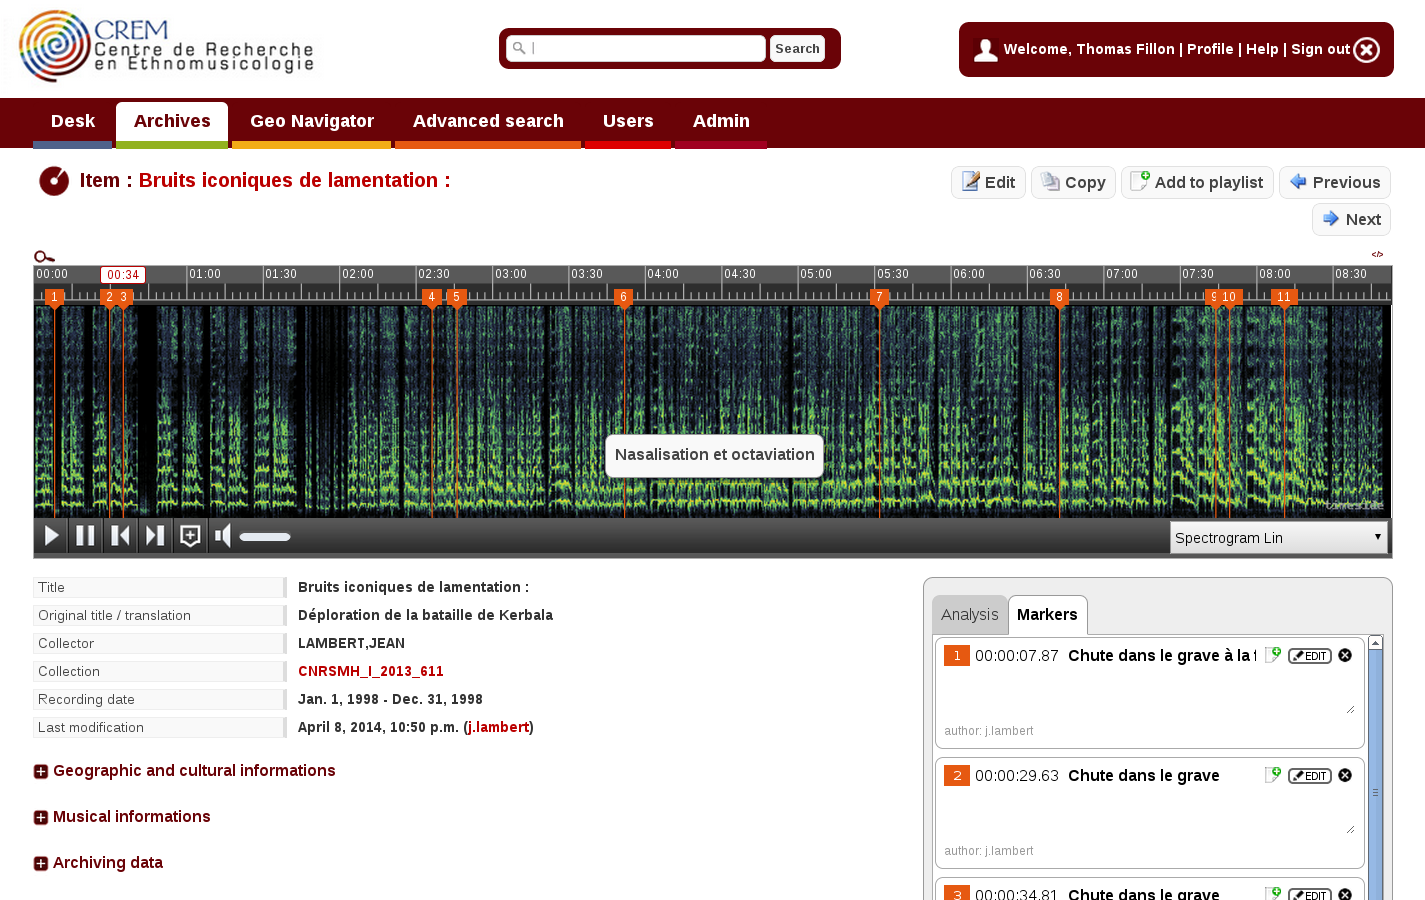
\includegraphics[width=8cm]{../../Common/img/telemeta_screenshot_en_2.png}
  \caption{The Telemeta platform deployed for the CNRS-CREM sound archives}
\label{fig:telemeta}
\end{figure}


Telemeta relies on TimeSide for audio decoding, encoding and streaming methods.  Also it enables the users of the CREM sound archives to have access to many different automatic audio analysis (e.g. pitch, speech segmentation, music segmentation, polyphony detection, start of recording session for tape recorder, ...).




Through collaboration with academic research labs in computer science, speech processing and music information retrieval, new automatic analysis functionalities are brought to the platform regularly.


     
The Telemeta and TimeSide platform are available as open-source projects at the following addresses:
\begin{itemize}
\item Telemeta: \url{https://github.com/Parisson/Telemeta}
\item TimeSide: \url{https://github.com/Parisson/TimeSide}
\end{itemize}


\end{sloppypar}
\end{document}
